\documentclass{article}
\usepackage{graphicx}
\graphicspath{ {images/} }

%%%%%%%%%%%%%%%%%%%%%%%%%%%%%%%%%%%%%%%%%
% Lachaise Assignment
% Structure Specification File
% Version 1.0 (26/6/2018)
%
% This template originates from:
% http://www.LaTeXTemplates.com
%
% Authors:
% Marion Lachaise & François Févotte
% Vel (vel@LaTeXTemplates.com)
%
% License:
% CC BY-NC-SA 3.0 (http://creativecommons.org/licenses/by-nc-sa/3.0/)
% 
%%%%%%%%%%%%%%%%%%%%%%%%%%%%%%%%%%%%%%%%%

%----------------------------------------------------------------------------------------
%	PACKAGES AND OTHER DOCUMENT CONFIGURATIONS
%----------------------------------------------------------------------------------------



\usepackage{amsmath,amsfonts,stmaryrd,amssymb} % Math packages

\usepackage{enumerate} % Custom item numbers for enumerations

\usepackage[ruled]{algorithm2e} % Algorithms

\usepackage[framemethod=tikz]{mdframed} % Allows defining custom boxed/framed environments

\usepackage{listings} % File listings, with syntax highlighting
\lstset{
	basicstyle=\ttfamily, % Typeset listings in monospace font
}

%----------------------------------------------------------------------------------------
%	DOCUMENT MARGINS
%----------------------------------------------------------------------------------------

\usepackage{geometry} % Required for adjusting page dimensions and margins

\geometry{
	paper=a4paper, % Paper size, change to letterpaper for US letter size
	top=2.5cm, % Top margin
	bottom=3cm, % Bottom margin
	left=2.5cm, % Left margin
	right=2.5cm, % Right margin
	headheight=14pt, % Header height
	footskip=1.5cm, % Space from the bottom margin to the baseline of the footer
	headsep=1.2cm, % Space from the top margin to the baseline of the header
	%showframe, % Uncomment to show how the type block is set on the page
}

%----------------------------------------------------------------------------------------
%	FONTS
%----------------------------------------------------------------------------------------

\usepackage[utf8]{inputenc} % Required for inputting international characters
\usepackage[T1]{fontenc} % Output font encoding for international characters

% \usepackage{XCharter} % Use the XCharter fonts

%----------------------------------------------------------------------------------------
%	COMMAND LINE ENVIRONMENT
%----------------------------------------------------------------------------------------

% Usage:
% \begin{commandline}
%	\begin{verbatim}
%		$ ls
%		
%		Applications	Desktop	...
%	\end{verbatim}
% \end{commandline}

\mdfdefinestyle{commandline}{
	leftmargin=10pt,
	rightmargin=10pt,
	innerleftmargin=15pt,
	middlelinecolor=black!50!white,
	middlelinewidth=2pt,
	frametitlerule=false,
	backgroundcolor=black!5!white,
	frametitle={Command Line},
	frametitlefont={\normalfont\sffamily\color{white}\hspace{-1em}},
	frametitlebackgroundcolor=black!50!white,
	nobreak,
}

% Define a custom environment for command-line snapshots
\newenvironment{commandline}{
	\medskip
	\begin{mdframed}[style=commandline]
}{
	\end{mdframed}
	\medskip
}

%----------------------------------------------------------------------------------------
%	FILE CONTENTS ENVIRONMENT
%----------------------------------------------------------------------------------------

% Usage:
% \begin{file}[optional filename, defaults to "File"]
%	File contents, for example, with a listings environment
% \end{file}

\mdfdefinestyle{file}{
	innertopmargin=1.6\baselineskip,
	innerbottommargin=0.8\baselineskip,
	topline=false, bottomline=false,
	leftline=false, rightline=false,
	leftmargin=2cm,
	rightmargin=2cm,
	singleextra={%
		\draw[fill=black!10!white](P)++(0,-1.2em)rectangle(P-|O);
		\node[anchor=north west]
		at(P-|O){\ttfamily\mdfilename};
		%
		\def\l{3em}
		\draw(O-|P)++(-\l,0)--++(\l,\l)--(P)--(P-|O)--(O)--cycle;
		\draw(O-|P)++(-\l,0)--++(0,\l)--++(\l,0);
	},
	nobreak,
}

% Define a custom environment for file contents
\newenvironment{file}[1][File]{ % Set the default filename to "File"
	\medskip
	\newcommand{\mdfilename}{#1}
	\begin{mdframed}[style=file]
}{
	\end{mdframed}
	\medskip
}

%----------------------------------------------------------------------------------------
%	NUMBERED QUESTIONS ENVIRONMENT
%----------------------------------------------------------------------------------------

% Usage:
% \begin{question}[optional title]
%	Question contents
% \end{question}

\mdfdefinestyle{question}{
	innertopmargin=1.2\baselineskip,
	innerbottommargin=0.8\baselineskip,
	roundcorner=5pt,
	nobreak,
	singleextra={%
		\draw(P-|O)node[xshift=1em,anchor=west,fill=white,draw,rounded corners=5pt]{%
		Question \theQuestion\questionTitle};
	},
}

\newcounter{Question} % Stores the current question number that gets iterated with each new question

% Define a custom environment for numbered questions
\newenvironment{question}[1][\unskip]{
	\bigskip
	\stepcounter{Question}
	\newcommand{\questionTitle}{~#1}
	\begin{mdframed}[style=question]
}{
	\end{mdframed}
	\medskip
}

%----------------------------------------------------------------------------------------
%	WARNING TEXT ENVIRONMENT
%----------------------------------------------------------------------------------------

% Usage:
% \begin{warn}[optional title, defaults to "Warning:"]
%	Contents
% \end{warn}

\mdfdefinestyle{warning}{
	topline=false, bottomline=false,
	leftline=false, rightline=false,
	nobreak,
	singleextra={%
		\draw(P-|O)++(-0.5em,0)node(tmp1){};
		\draw(P-|O)++(0.5em,0)node(tmp2){};
		\fill[black,rotate around={45:(P-|O)}](tmp1)rectangle(tmp2);
		\node at(P-|O){\color{white}\scriptsize\bf !};
		\draw[very thick](P-|O)++(0,-1em)--(O);%--(O-|P);
	}
}

% Define a custom environment for warning text
\newenvironment{warn}[1][Warning:]{ % Set the default warning to "Warning:"
	\medskip
	\begin{mdframed}[style=warning]
		\noindent{\textbf{#1}}
}{
	\end{mdframed}
}

%----------------------------------------------------------------------------------------
%	INFORMATION ENVIRONMENT
%----------------------------------------------------------------------------------------

% Usage:
% \begin{info}[optional title, defaults to "Info:"]
% 	contents
% 	\end{info}

\mdfdefinestyle{info}{%
	topline=false, bottomline=false,
	leftline=false, rightline=false,
	nobreak,
	singleextra={%
		\fill[black](P-|O)circle[radius=0.4em];
		\node at(P-|O){\color{white}\scriptsize\bf i};
		\draw[very thick](P-|O)++(0,-0.8em)--(O);%--(O-|P);
	}
}

% Define a custom environment for information
\newenvironment{info}[1][Info:]{ % Set the default title to "Info:"
	\medskip
	\begin{mdframed}[style=info]
		\noindent{\textbf{#1}}
}{
	\end{mdframed}
}
 % Include the file specifying the document structure and custom commands

										%-------------------------------%
										%	ASSIGNMENT INFORMATION		%
										%-------------------------------%

\title{LIS4031: Project \#2} % Title of the assignment

\author{Jose Carlos Archundia Adriano - Carlos Andres Reyes Evangelista - Erick Siordia Nagaya\\ \texttt{jose.archundiaao@udlap.mx - carlos.reyesea@udlap.mx - erick.siordiana@udlap.mx}} % Authors name and email addresses

\date{Universidad de las Am\'ericas  Puebla --- \today} % University, school and/or department name(s) and a date

										%-------------------------------%
										%			DOCUMENT			%
										%-------------------------------%

\begin{document}

\maketitle % Print the title

%-------------------------------%
%		INTRODUCTION			%
%-------------------------------%
\section{Introduction} % Unnumbered section
Today it is very common for people to make use of data stored in the web, however, sometimes finding that data turns out to be complicated and/or very time consuming. In order to solve this problem, \textit{web crawlers} can be used to automate the process of finding and downloading websites that contain relevant data or information.
Specialized areas, such as linguistics, can also make use of \textit{web crawlers} to solve problems.
In this project, we take on the challenge of extracting data from the web to build a list of German words that are derived from English. Specifically, the project uses the \textbf{duden.de} website to find the data of each word procured from a list of German words. The crawler will be responsible for downloading the website corresponding to each German word so they can be analyzed by a program that will check if the word has an English origin or not. This word list will be used later to compute the percentage of words that are derived from English in an article procured from a collection of documents written in german.

\section{Description}
The proposed solution to the challenge explained previously is a program that crawls each word's corresponding entry in \textbf{duden.de} to then analyze it and determine if it has an English origin or not. The program is composed of 3 main parts: the web crawler, the processing threads, and the document analyzer.
The crawler is a program that, for each word in the list of German words, accesses its data site and obtains its HTML content. Then, it stores a part of the HTML content in a shared-memory queue. This queue will then be analyzed by the processing threads in our program. This part is composed by \textit{n} independent threads that are constantly dequeueing the sites from the shared-memory queue in order to analyze the HTML chunk and determine if in the check contains a \textit{Herkunft}, or origin, section, and if the \textit{Herkunft} contains the word "englisch", the german spelling of \textit{english}. If the word is contained in the \textit{Herkunft} section, it is considered to have an English origin, and is written to a file containing all English-derived German words. It is important to note that the crawler will always be enqueueing new sites to the shared-memory queue as long as there are words remaining in the list of German words, and the independent threads will be constantly dequeueing them from the shared-memory queue.
Finally, the last part is the document analyzer, which uses the list of English-derived words generated by the threads in order to compute the percentage of English-derived words that are present in an article chosen by the user from the collection of German articles. In order to achieve this task, this program simply counts the total number of words in the article, as well as the amount of words in the article that exist in our list of English-derived words.

\section{Methodology}
As stated before, the focus of this project is to identify the words that have an English origin from a set of German words. To do this, the first thing we require is to have a list of German words to query the web dictionary \textbf{duden.de}. This set of words was divided into several parts, with each one being assigned to a different teamworking on this same project. This was done because the crawling of each word takes time, and crawling all of them would have taken weeks or even months of crawling.\\
After having the portion of the words set assigned, the next task was to implement the crawler by analysing the patterns that identify each different type of page on the site. Thanks to this analysis, a pattern was discovered that consists on checking the number of "lead" elements in the HTML code of the sites. Four cases were identified: A case where the site contained several word suggestions for your query, another that displayed a text saying \textit{Did you mean to say...} and a suggested word, a case when the site automatically redirects you to a suggested word if the introduced one is not found, and finally, the last case was when the page simply displayed a message saying that the word was not found.
The only case that was selected for processing was the one which has several suggested words because in the other cases, there is the probability that the word that the site proposes is not the one the program was looking for. To process this word site an analysis is on the HTML structure of the site in order to know if it contains the word the program is looking for. Finally, the last thing done in the crawler is the transfer of the HTML code required to the shared stack for the independent threads to analyze.
\\
After this, the code to implement the threads and the HTML processing was implemented. To do this, the class \textit{pThread} was written. This inherits the Python's \textbf{Thread} class, which has attributes to receive the output file stream, the reference of the shared queue, and objects to maintain the concurrency of the program. The class also contains the method \textit{run()} to continuously check if there are documents in the queue. If there are, the HTML code is obtained from the queue and analysed to know if the \textit{Herkunft} section contains the "englisch" word.
After several tests, the crawlers was left running on 5 different computers for several hours to obtain all the website entries of the words in the assigned set.
The final part of the project was to implement a program to compare the German articles found in the \textbf{articles.csv} document. For this, a brief menu is displayed for the user to select one option. The options are to select a random number of articles, or for the user to input a specific article number to analyze.

\section{Implementation}
The actual implementation of this project consists of two independent programs written in the programming language \textit{Python}:
\begin{itemize}
	\item[$-$] Web Crawler: This program is responsible for sending requests to the German dictionary and discerning if the requested word comes from the English language. As output, it generates a list that includes each word found by the crawler to have an English origin.
	\item[$-$] Document analyzer: This program uses the output from the previous program to determine the ratio of the words in each article that come from English when given a set of articles written in German.
\end{itemize}

The Web Crawler itself is divided into two modules as mentioned before: the \textit{main thread} which handles the HTTP requests, and the \textit{processing threads} which analyses the results of the main thread's requests.


As might be noted, these two processes are connected in a \textbf{Producer - Consumer} approach. The main thread \textit{produces} by enqueueing in a shared-memory queue a chunk of HTML from the source of each word that has a page in the \textit{Duden} dictionary. The processing threads are started by the main thread before it begins to work. They are kept in a idle-state as long as the queue is empty, only waking up to peek at the queue. If the queue is empty then they sleep again, otherwise, they try to acquire a \textit{lock} corresponding to the queue in order to read and write from it. If they manage to obtain the lock, they will dequeue one element of the shared queue for its further processing, \textit{consuming} the HTML chunk, and release the lock immediately.

To clarify this concept, both algorithms will be further explained step by step with pseudo-code.

\begin{center}
	\begin{minipage}{0.8\linewidth} % Adjust the minipage width to accommodate for the length of algorithm lines
		\begin{algorithm}[H]
			\KwIn{$wordsFile$, a plain-text file with a german word in each line}  % Algorithm inputs
			\KwResult{$queue$, a shared-memory queue that will be constantly updated for the parallel threads to obtain sources to analyze} % Algorithm outputs/results
			\medskip
			queue = Queue()\\
			queueLock = fileLock = Lock()\\
			\medskip
			startThreads()\\
			\medskip
			\For{word in wordsFile}{
				\textit{//Perform an HTTP request to emulate a "search" in the dictionary and retrieve a parser for its source}\\
				document = getHTMLdocument(dudenURL + word)\\
				\medskip
				\textit{//If it redirects to a valid page}\\
				\If{document}{
					pageType = getPageType(document)\\
					\medskip
					\textit{//Check if the obtained page holds links to word-page}\\
					\If{pageType == TypesOfPage.links}{
						\textit{//Attempt to locate a link within the links-page to a page whose word matches the searched one}\\
						wordPage = getWordPage(document, word)\\
						\medskip
						\textit{//If the program was able to find a link to a word-page}\\
						\If{wordPage}{
							\textit{//Perform an HTTP request to that page and enqueue it for further processing}\\
							wordDocument = getHTMLdocument(document)\\
							queueLock.acquire()\\
							queue.put(wordDocument)\\
							queueLock.release()\\
						}
					}
				}
			}
			\caption{\texttt{Crawler}} % Algorithm name
			\label{alg:fastTwoSum}   % optional label to refer to
		\end{algorithm}
	\end{minipage}
\end{center}

The only \textit{ad-hoc} details to note here are that:
\begin{itemize}
	\item The user-defined function $getHTMLdocument()$ receives an URL as an argument, converts it to a \textit{safe URL}, i.e., casting Unicode characters into ASCII escape codes, performs an HTTP request to the latter, and returns a parser for the HTML obtained or an error if the HTTP request was unsuccessful.
	\item The user-defined function $getWordPage()$ iterates through all the links provided by a \textit{"links-page"} and tries to find a match between the link the page offers and the word that the program is searching for. If it finds one, it will return its relative link, otherwise it will return an error state.
	\item The $queueLock$ lines are extremely important for avoiding \textit{race conditions} with the resources shared among parallel threads. The operations $acquire()$ and $release()$ ensure that, at that exact moment, no other thread is reading or writing to the same resource.
	\item The german dictionary \textit{Duden} returns different types of pages depending on its own search of a given word. The ones that are taken into account are listed below along with its description:
	\begin{itemize}
		\item[-] Type of page: \textit{links}. This page is returned when the word exiests in the dictionary or is contained in an existing word. This is the only case that will make a word be considered valid because it is the only case in which the word might possibly be found. Example: https://www.duden.de/suchen/dudenonline/computer
		\item[-] Type of page: \textit{didYouMean}. This page is returned when the input word is an anagram of an existing one so the site suggests a link of a similarly written word. This case is discarded because if the site is suggesting a different wrod, it is because it did not find a match. Example: https://www.duden.de/suchen/dudenonline/lückenlosen
		\item[-] Type of page: \textit{notFoundBut}. This page is returned when the input word was not found as it was written, but a very likely match was found, so it automatically redirects the user to that matched word. It is ignored because similarity does not imply equality, and given that it \textbf{did not} find the one searched, then this is not a link to the searched word. Example: \\https://www.duden.de/suchen/dudenonline/facelifting?ls=faceliting\&s=facelifting
		\item[-] Type of page: \textit{notFound}. This page is presented when the word was not found and no link is suggested. It is ignored by our program. Example: \\https://www.duden.de/suchen/dudenonline/lückenlosen
		\item[-] Type of page: \textit{wordPage}. This kind of page is the one holds a word's entry in the dictionary including its meaning, part of speech, and of course, origin. Example: \\https://www.duden.de/rechtschreibung/Computer
	\end{itemize}
\end{itemize}













The counterpart to the crawler, the processing thread, is as follows:

\begin{center}
	\begin{minipage}{0.8\linewidth} % Adjust the minipage width to accommodate for the length of algorithm lines
		\begin{algorithm}[H]

			\KwIn{$queue$, a shared-memory queue that will be constantly updated for the parallel threads to obtain sources to analyse} % Algorithm outputs/results
			\KwResult{$englishHerkunftWords$, a plain-text file with a german word of english origin in each line; $lastProcessedWord$, a plain-text file with the last word processed by the program}  % Algorithm inputs
			\medskip
			running = True
			\medskip
			processingThread()
				\medskip
				\textit{//Initializes the thread with pointers to the different resources}\\
				function init(queue, queueLock, documentStream, documentStreamLock)\\
				\medskip
				\textit{//Signal thread to stop}\\
				function signalStop()\\
					running = False
				\medskip
				\textit{//Executed when thread is run}
				function run()\\
					\While{running}{
					\textit{//Control flag for checking document retrieved from queue}
					flag = False\\
					document = null\\

					queueLock.acquire()\\
					\If{not queue.empty}{
						document = queue.dequeue()\\
						flag = ture\\
						}
					\textit{//Release queue lock so anotherpart of the program can access it}
					queueLock.release()\\
					\medskip
					\If{flag}{
						\textit{//split doc into required components}\\
						title = document.getTitleElement()\\
						herkunft = document.getHerkunftElement\\
						\textit{//Check if word originates from english}\\
						engFlag, word = processDocument(title, herkunft)\\
						\medskip
						\If{engFlag}{
							\textit{//acquire document stream lock and write}\\
							documentStreamLock.acquire()\\
							documentStream.write(word)\\
							lastProcessedWord.write(word)\\
							documentStreamLock.release()\\
						}
						\textit{//Tell inactive thread to sleep}
						time.sleep(random())
					}
				}
				\medskip
				\textit{//Function scans document chunks for english origin}
				function processDocument(title, herkunft)\\
						word = title.scanForWord()\\
						\If{herkunft}{
							englishFlag = herkunft.searchFor("englisch")\\
							\If{englishFlag}{
								return True, word\\
								}
						}
						return False, word\\
			\caption{\texttt{Processing Thread}} % Algorithm name
		\end{algorithm}
	\end{minipage}
\end{center}

Some things to note are:
\begin{itemize}
	\item The lock for the documentStream and lastProcessedWord files are shared
	\item The threads dequeue HTMl chucks from the shared-memory queue. In our implementation, these are instances of HTML parser objects with just the required chunk.
\end{itemize}

For the implementation of the second program, the document analyser, the list of german words with english origin produced by the previous program is used. As shown in the following pseudo code, the ratio of the english-derived words in an article is computed by dividing the length of the set that is the intersection of the english derived-words and the article's words, by the length of the set of the article's words.
\begin{center}
	\begin{minipage}{0.8\linewidth} % Adjust the minipage width to accommodate for the length of algorithm lines
		\begin{algorithm}[H]
			\KwIn{$articles$, the path to the collection of articles in German; $englishWords$, the path to the list of English-derived words; $index$, the index of the article to analyse.}  % Algorithm inputs
			\KwResult{$ratio$, a double number that represents the ratio of german-derived words to the total number of words in the article.} % Algorithm outputs/results
			\medskip
			english\_derived\_words = load\_word\_list(englishWords)\\
			articles = load\_articles(articles)\\
			\medskip

			desired\_article = articles[index]

			detected\_words = list()

			\For {word in english\_derived\_words} {
				\If{word in article} {
					detected\_words.append(word)
				}
			}

			return len(detected\_words)/len(article)

			\caption{\texttt{Document Analyser}} % Algorithm name
			\label{alg:fastTwoSum}   % optional label to refer to
		\end{algorithm}
	\end{minipage}
\end{center}

\section{Results}
While implementing our solution for the web crawler, we came across some inconsistencies in the design of the website \textbf{dunden.de}. One such case was where a word is not found in the dictionary. Usually, the website will say the word is not found and provide a list of alternatives. Other times, it will only say the page for that word doesn't exist. Very rarely, the page will also redirect to a similiar word. In order to combat this, and other inconsistencies in the page we designed our crawler to only deal with the following cases corresponding to the \textit{type of pages} described earlier:

\begin{itemize}
	\item Word is not found: corresponds to the \textit{notFound} type of page. Examples in \textit{figure 1} and \textit{figure 2}.\\
	\item Autocorrected word: corresponds to the \textit{notFoundbut} type of page. Examples in \textit{figure 3} and \textit{figure 4}.
	\item Word not found, list of alternatives provided: corresponds to the \textit{didYouMean} type of page. Examples in \textit{figure 5} and \textit{figure 6}.
	\item Word found: corresponds to the \textit{wordPage} type of page. Examples in \textit{figure 7} and \textit{figure 8}.
\end{itemize}

The first three types of pages are discarded by our crawler, as can be seen in \textit{figures 1, 3, and 5}.\\
The last case, \textit{wordPage}, is processed by enqueueing a chunk of HTML to our shared-memory queue to be interpreted by our processing threads.
Three things can happen in this case:
\begin{itemize}
	\item The page has no \textit{Herkunft} section. We stop processing and the word is discarded, \textit{figure 5}.
	\item The page has a \textit{Herkunft} section, but it does not contain the word \textit{englisch}. The word is discarded, \textit{figure 10}.
	\item The page has a \textit{Herkunft} section that contains the word \textit{englisch}. The word is saved in order to be written to the file as soon as the thread is able to acquire the documentStream lock,\textit{figure 5}.\\
\end{itemize}

Our results indicate that the vast majority of word in our German word list do not have an English origin. This is partly due to the website not indicating that words derived from other words with an english origin have an english origin. Another reason for this is that our original German words listis not exhaustive.


\section{Conclusion}Through the development of this project, a real application for web crawlers was implemented, and with this, the usefulness that this kind of software provides to the Information Retrieval area was also explored. It is also thanks to this project that the team had to design and implement several \textit{ad-hoc} solutions to the challenges that the crawling of the required data implied, like the classification of different data sites and the handling of errors like time-outs and broken links. We also exploredoptimization solutions, such as the threaded processing of the HTML responses, in order to try to speed up the crawling process. We are able to retrieve a list of all the words in our input list of German words that have an English origin. Our implementation is able to handle any exceptions or inconsistencies the website may have and retrievs the information that we are looking for. Although our program functions perfectly, there are some features of the program could be improved, like the handling of the different types of retrieved pages, and the searching for derived words in the \textbf{duden.de} site instead of only perfect matches. This would allow us to compensate for inconsistencies in the website's design and retrieve an exhaustive list of German words with english origin.

\section{References}
Croft, W., Metzler, D. and Strohman, T. (2009). \textit{Information retrieval in practice.} Upper Saddle River, N.J.: Pearson Education.

\section{Apendix}

\begin{figure}[h]
	\caption{Word not found - program}
	\centering
	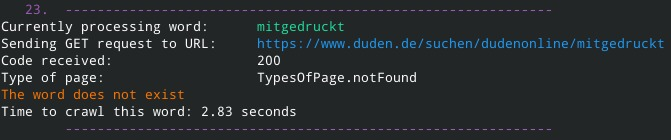
\includegraphics[scale=0.5]{1}
\end{figure}

\begin{figure}[h]
	\caption{Word not found - website}
	\centering
	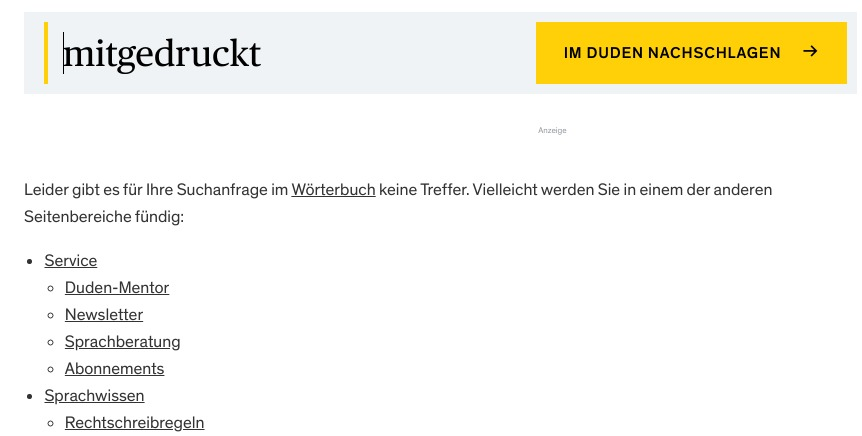
\includegraphics[scale=0.5]{2}
\end{figure}


\begin{figure}[h]
	\caption{Autosuggested Correction - program}
	\centering
	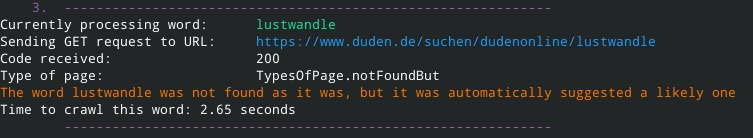
\includegraphics[scale=0.5]{3}
\end{figure}

\begin{figure}[h]
	\caption{Autosuggested Correction - website}
	\centering
	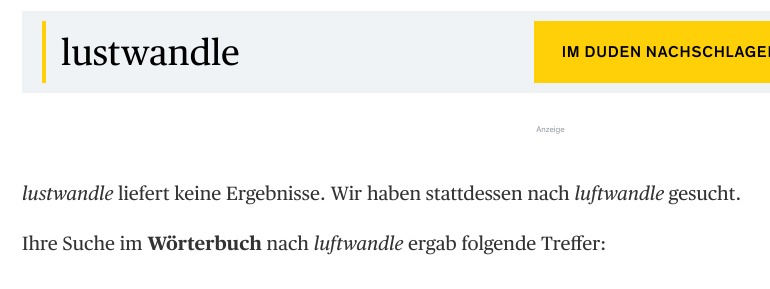
\includegraphics[scale=0.5]{4}
\end{figure}


\begin{figure}[h]
	\caption{Found list of alternatives - program}
	\centering
	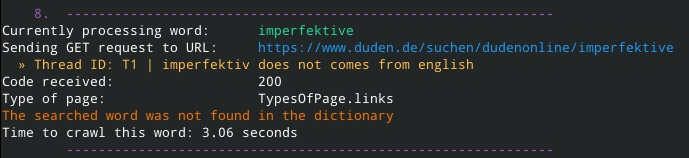
\includegraphics[scale=0.5]{5}
\end{figure}

\begin{figure}[h]
	\caption{Found list of alternatives - website}
	\centering
	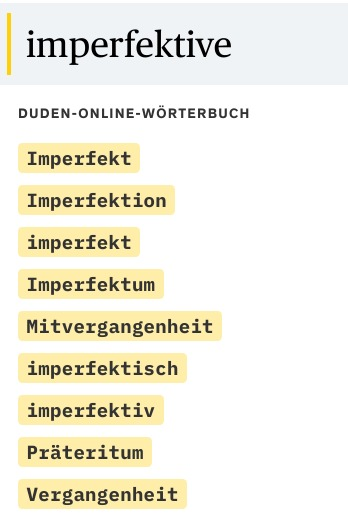
\includegraphics[scale=0.5]{6}
\end{figure}


\begin{figure}[h]
	\caption{Word found - program}
	\centering
	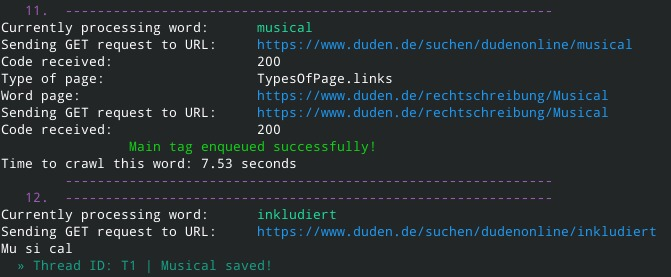
\includegraphics[scale=0.5]{7}
\end{figure}

\begin{figure}[h]
	\caption{Word found - website}
	\centering
	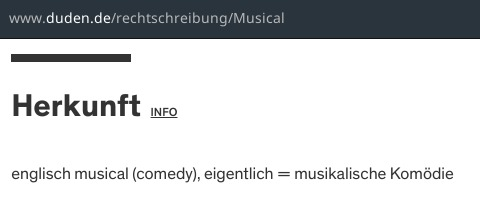
\includegraphics[scale=0.5]{8}
\end{figure}


%----------------------------------------------------------------------------------------
\end{document}
